
使用CMake最常见的方式是通过命令行(CLI)。本节中,将了解如何使用CLI执行最基本的CMake操作。

与CMake CLI的交互可以通过在终端中输入CMake命令来完成,假设安装了CMake,并且CMake可执行文件包含在系统的PATH变量(或等效变量)中。就可以通过在终端中不带任何参数地执行\texttt{cmake}来进行验证:

\begin{center}
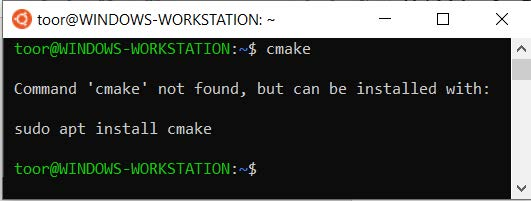
\includegraphics[width=0.8\textwidth]{content/1/chapter2/images/1.jpg}\\
图2.1 调用cmake命令
\end{center}

若终端抱怨缺少命令,那么需要安装CMake或者将其可执行文件的目录添加到系统的PATH变量中。关于如何向系统的PATH变量添加路径,请参考操作系统指南。

在安装CMake并将其添加到PATH变量后(如果需要),应该测试CMake是否可用。可以在命令行中执行的最基本命令是\texttt{cmake -{}-version},它允许您检查CMake的版本。

\begin{center}
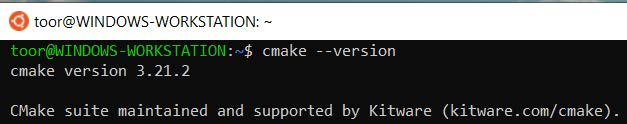
\includegraphics[width=1.\textwidth]{content/1/chapter2/images/2.jpg}\\
图2.2 在终端中查看CMake的版本
\end{center}

CMake版本将以<maj.min.rev>的形式输出一个版本字符串,其中包含您在系统上安装的CMake的版本号。

\begin{tcolorbox}[colback=webgreen!5!white,colframe=webgreen!75!black,title=Note]
若版本与安装的不匹配,可能系统中已经安装了多个CMake。由于本书包含了为CMake 3.21及以上版本编写的示例,因此建议在进一步讨论之前修复该问题。
\end{tcolorbox}

安装CMake之后,应该安装构建系统和编译器。对于类似Debian的操作系统(例如,Debian和Ubuntu),这可以通过发出\texttt{sudo apt install build-essential}命令轻松完成,这个包包含gcc、g++和make。

CLI的用法将在Ubuntu 20.04环境中说明,在其他环境中的用法也是一样的。这些边缘情况会在后面介绍。

\subsubsubsection{2.2.1\hspace{0.2cm}了解CMake命令行的基本操作}

下面列出了使用CMake命令行应该了解的三件事情:

\begin{itemize}
\item 
配置

\item 
构建

\item 
安装
\end{itemize}

学习了基础知识之后,将能够构建和安装任何CMake项目。

\hspace*{\fill} \\ %插入空行
\noindent
\textbf{通过命令行配置项目}

要通过命令行配置CMake项目,可以使用\texttt{CMake -G "Unix Makefiles" -S  -B <output\_directory>}的方式。\texttt{-S}参数用于指定要配置的CMake项目,而\texttt{-B}参数用于指定配置输出目录。最后,\texttt{-G}参数指定将用于生成构建系统的生成器,配置过程的结果将写入\texttt{<output\_directory>}。

在项目根构建目录中配置我们书中的示例项目:

\begin{center}
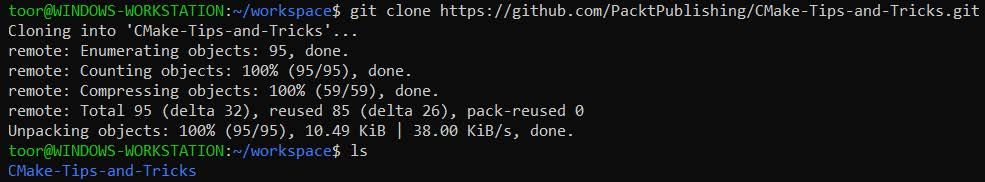
\includegraphics[width=1.\textwidth]{content/1/chapter2/images/3.jpg}\\
图2.3 克隆示例代码存储库
\end{center}

\begin{tcolorbox}[colback=webgreen!5!white,colframe=webgreen!75!black,title=重要Note]
项目必须存在于环境中。若没有,需要在Git在终端中执行\texttt{git clone \url{https://github.com/PacktPublishing/CMake-Best-Practices.git}}。
\end{tcolorbox}

现在进入CMake-Best-Practices目录,使用\texttt{cmake -G "Unix Makefiles" -S . -B ./build}:

\begin{center}
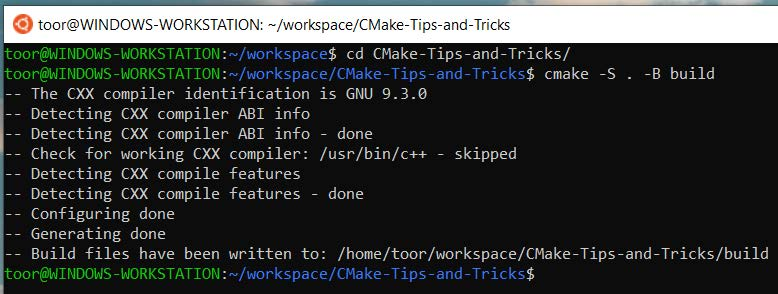
\includegraphics[width=1.\textwidth]{content/1/chapter2/images/4.jpg}\\
图2.4 使用CMake配置示例代码
\end{center}

这个命令就像对CMake说,使用"Unix Makefiles" (\texttt{-G "Unix Makefiles"})生成器在当前目录(\texttt{-S .})生成CMake项目的构建系统(\texttt{-B ./build})目录。

CMake将设置源文件夹为当前文件夹中的项目。当我们省略构建类型时,CMake使用Debug构建类型(项目默认的\texttt{CMAKE\_BUILD\_TYPE})。

在后续章节中,我们将学习配置步骤中使用的基本设置。

\hspace*{\fill} \\ %插入空行
\noindent
\textbf{修改构建类型}

CMake默认不假定任何构建类型。为了设置构建类型,必须在配置阶段提供一个名为\texttt{CMAKE\_BUILD\_TYPE}的变量,变量必须以\texttt{-D}作为前缀。

要获得Release版本,而不是Debug版本,在配置命令中添加\texttt{CMAKE\_BUILD\_TYPE}变量。如前所述,该命令为:\texttt{cmake -G "Unix Makefiles" -DCMAKE\_BUILD\_TYPE:STRING=Release -S . -B ./build}。

\begin{tcolorbox}[colback=webgreen!5!white,colframe=webgreen!75!black,title=Note]
\texttt{CMAKE\_BUILD\_TYPE}变量只对单个配置生成器有意义,例如Unix Makefiles和Ninja。在多个配置生成器中,例如Visual Studio,构建类型是一个构建时参数而,不是一个配置时参数,因此不能通过使用\texttt{CMAKE\_BUILD\_TYPE}参数来配置。
\end{tcolorbox}

\hspace*{\fill} \\ %插入空行
\noindent
\textbf{更换生成器类型}

根据不同的环境,CMake会在默认情况下尝试选择合适的生成器。要显式指定生成器,\texttt{-G}参数必须提供有效的生成器名称。例如,若想使用Ninja作为构建系统,而不是make,可以这样:

\begin{tcblisting}{commandshell={}}
cmake -G "Ninja" -DCMAKE_BUILD_TYPE:STRING=Debug -S . -B ./
build
\end{tcblisting}

输出的信息应如下图所示:

\begin{center}
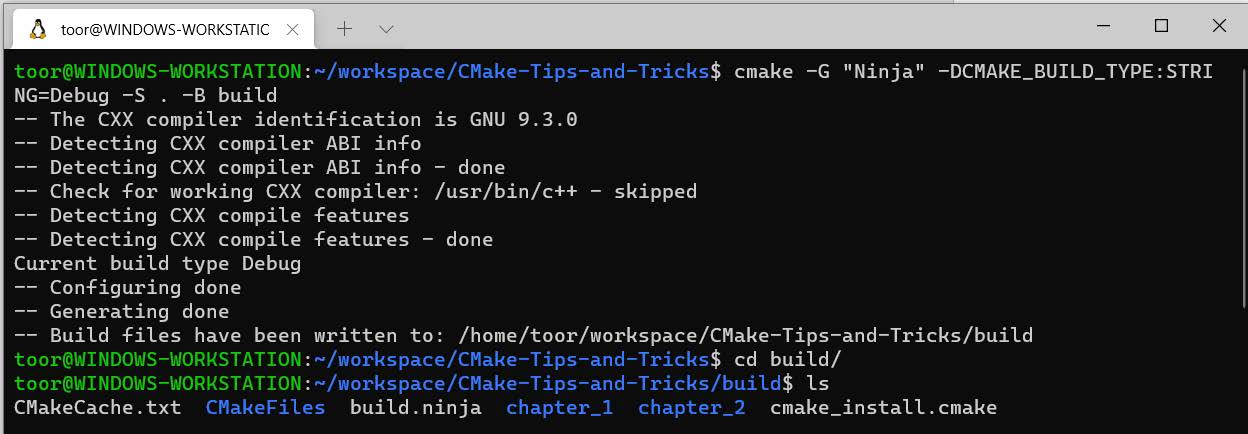
\includegraphics[width=1.\textwidth]{content/1/chapter2/images/5.jpg}\\
图2.5 检查CMake的Ninja生成器输出
\end{center}

这将导致CMake生成Ninja的构建文件,而不是生成makefile文件。

为了查看环境中所有可用的生成器类型,可使用\texttt{cmake -{}-help}。可用的生成器将在帮助文本生成器部分的末尾列出,如下所示:

\begin{center}
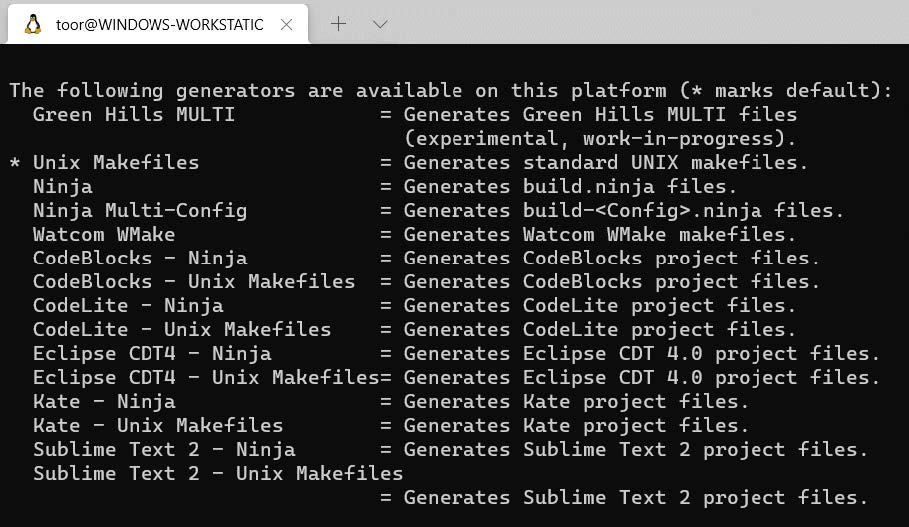
\includegraphics[width=0.6\textwidth]{content/1/chapter2/images/6.jpg}\\
图2.6 可用生成器列表
\end{center}

带有星号的生成器是当前环境的默认值。

\hspace*{\fill} \\ %插入空行
\noindent
\textbf{修改编译器}

CMake中,编译器可以通过\texttt{CMAKE\_<LANG>\_COMPILER}来指定。为了改变编译器,必须在配置命令中提供\texttt{CMAKE\_<LANG>\_COMPILER}。对于C/C++项目,通常覆盖的是\texttt{CMAKE\_C\_COMPILER}(C编译器)和\texttt{CMAKE\_CXX\_COMPILER}(C++编译器)。编译器标志由\texttt{CMAKE\_<LANG>\_FLAGS}控制。此变量可用于保存与配置无关的编译器标志。

例如,尝试使用g++-10作为C++编译器,但它不是默认编译器:

\begin{tcblisting}{commandshell={}}
cmake -G "Unix Makefiles" -DCMAKE_CXX_COMPILER=/usr/bin/g++-10 -S .  
  -B ./build
\end{tcblisting}

可以看到使用了g++-10,而不是系统默认的编译器g++-9:

\begin{center}
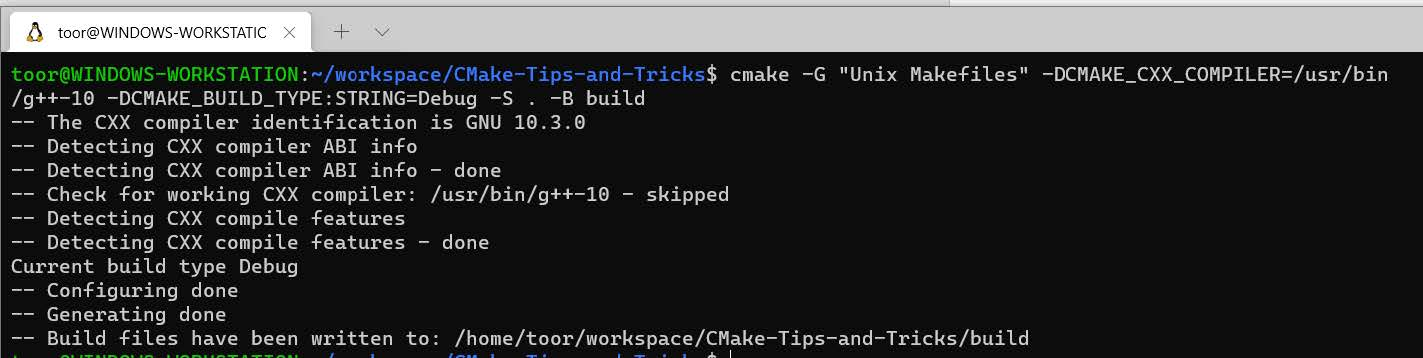
\includegraphics[width=1.\textwidth]{content/1/chapter2/images/7.jpg}\\
图2.7 使用不同的编译器配置项目(g++-10)
\end{center}

没有编译器规范的情况下,CMake更倾向于在这种环境下使用g++-9:

\begin{center}
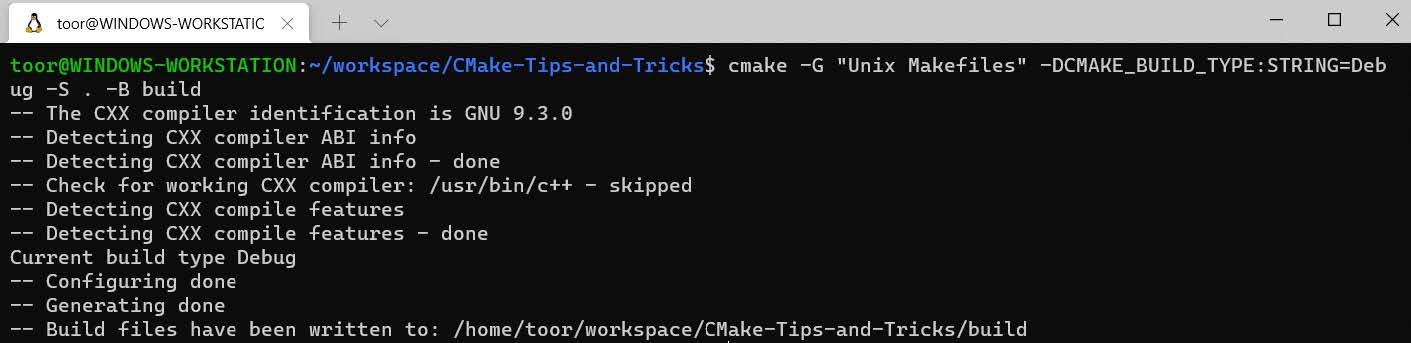
\includegraphics[width=1.\textwidth]{content/1/chapter2/images/8.jpg}\\
图2.8 不使用编译器配置的情况
\end{center}

\hspace*{\fill} \\ %插入空行
\noindent
\textbf{向编译器传递编译标志}

为了演示如何指定编译器标志,假设需要启用警告视为错误。这些行为在gcc工具链中分别用\texttt{-Wall}和\texttt{-Werror}编译器标志控制。因此,需要将这些标志传递给C++编译器:

\begin{tcblisting}{commandshell={}}
cmake -G "Unix Makefiles" -DCMAKE_CXX_FLAGS:STRING="-Wall
  -Werror" - S . B ./build S . -B ./build
\end{tcblisting}

可以看到命令中指定的标志(\texttt{-Wall}和\texttt{-Werror})在下面的例子中传递给了编译器:

\begin{center}
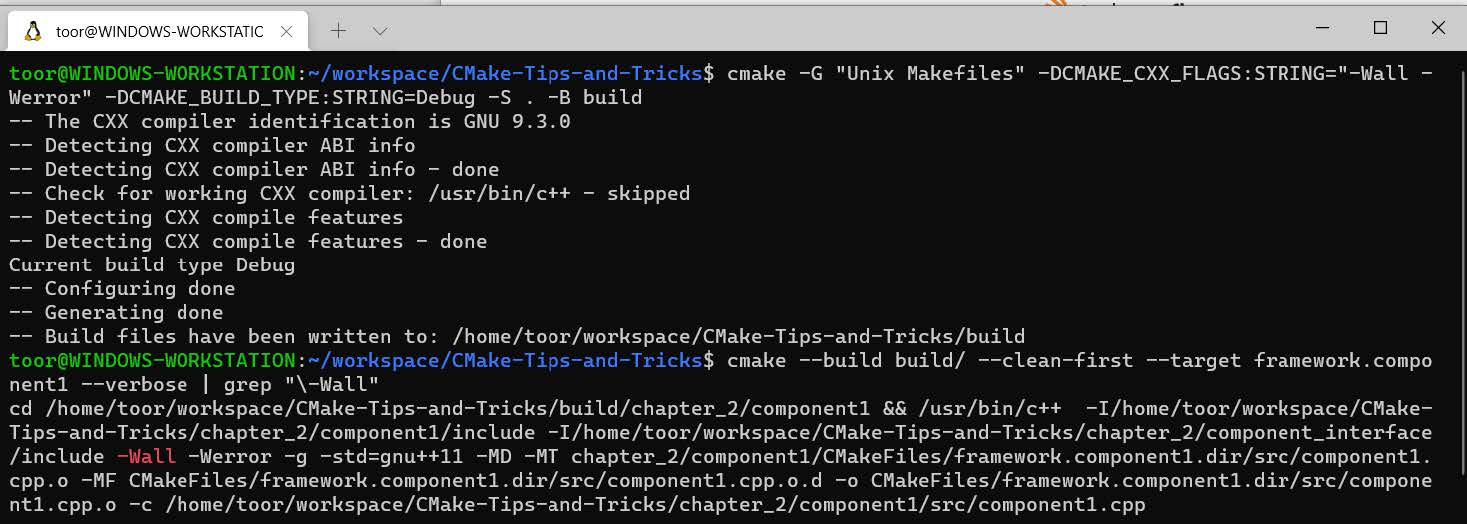
\includegraphics[width=1.\textwidth]{content/1/chapter2/images/9.jpg}\\
图2.9 向C++编译器传递标志
\end{center}

构建标志可以为每个构建类型定制,方法是在它们后面加上大写的构建类型字符串。有四个变量用于四个不同的构建类型,它们对于根据编译器标志指定构建类型非常有用。这些变量中指定的标志只在配置构建类型匹配时有效:

\begin{enumerate}
\item 
\texttt{CMAKE\_<LANG>\_FLAGS\_DEBUG}

\item 
\texttt{CMAKE\_<LANG>\_FLAGS\_RELEASE}

\item 
\texttt{CMAKE\_<LANG>\_FLAGS\_RELWITHDEBINFO}

\item 
\texttt{CMAKE\_<LANG>\_FLAGS\_MINSIZEREL}
\end{enumerate}

除了前面的例子外,若希望只在Release构建中将警告视为错误,可以使用构建类型特定的编译器标志。

下面是一个示例,演示了如何使用特定于构建类型的编译器标志:

\begin{tcblisting}{commandshell={}}
cmake -G "Unix Makefiles" -DCMAKE_CXX_FLAGS:STRING="-Wall
  -Werror" -DCMAKE_CXX_FLAGS_RELEASE:STRING="-O3" -DCMAKE_BUILD_
  TYPE:STRING=Debug -S . -B ./build
\end{tcblisting}

注意,前面的命令中有一个\texttt{CMAKE\_CXX\_FLAGS\_RELEASE}参数。只有当构建类型为Release时,这个变量中的内容才会传递给编译器。由于构建类型指定为Debug,可以看到传递给编译器的标志中没有\texttt{-O3}标志:

\begin{center}
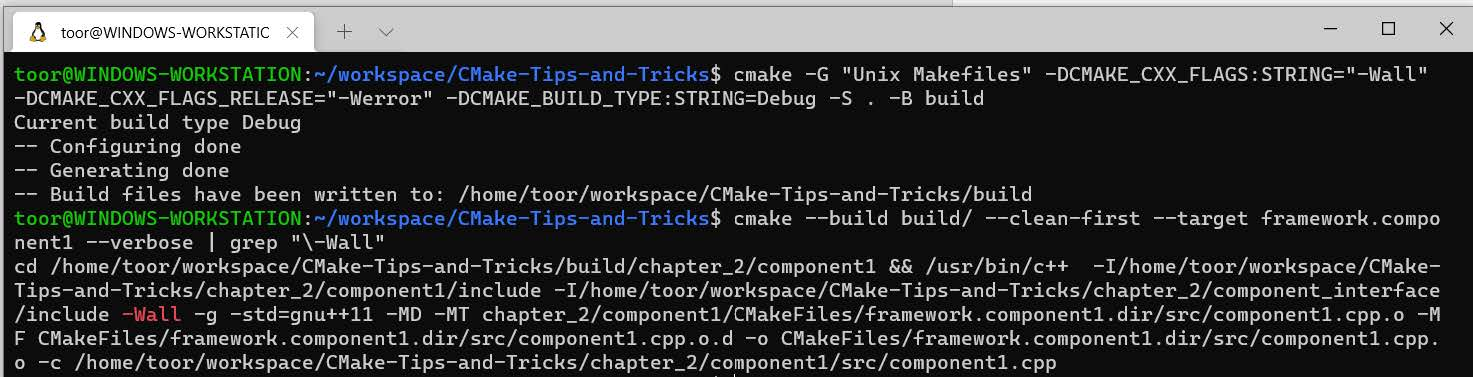
\includegraphics[width=1.\textwidth]{content/1/chapter2/images/10.jpg}\\
图2.10 根据构建类型指定标志——Debug版本中没有-O3标志
\end{center}

图2.10中,CMake发出一个关于指定,但未使用的变量的警告,\texttt{CMAKE\_CXX\_FLAGS\_RELEASE}。这确认了\texttt{CMAKE\_CXX\_FLAGS\_RELEASE}没有在Debug构建类型中使用。当构建类型指定为Release时,可以看到\texttt{-O3}标志:

\begin{tcblisting}{commandshell={}}
cmake -G "Unix Makefiles" -DCMAKE_CXX_FLAGS:STRING="-Wall
-Werror" -DCMAKE_CXX_FLAGS_RELEASE:STRING="-O3"
-DCMAKE_BUILD_TYPE:STRING= "Release" -S . -B ./build
\end{tcblisting}

相当于对CMake说,配置位于当前目录的CMake项目,使用“Unix Makefiles”生成器来构建/文件夹。对于所有构建类型,无条件地将\texttt{-Wall}标志传递给编译器。若构建类型是Release,也传递\texttt{-O3}标志。

以下是当构建类型设置为Release时命令的输出:

\begin{center}
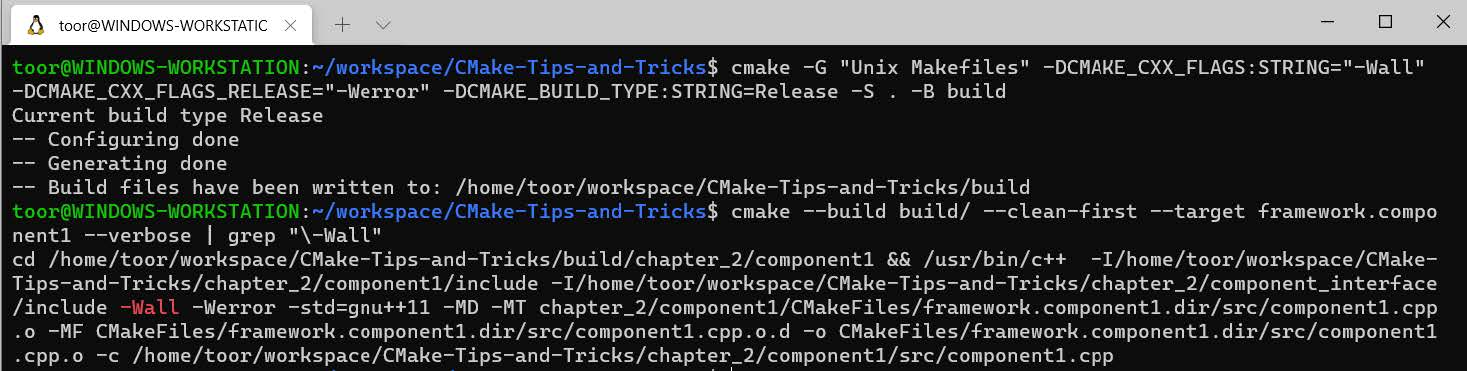
\includegraphics[width=1.\textwidth]{content/1/chapter2/images/11.jpg}\\
图2.11 根据构建类型指定标志——在Release版本中有\texttt{-O3}标志
\end{center}

In Figure 2.11, we can confirm that the -O3 flag is passed to the compiler as well. Be aware that even though RelWithDebInfo and MinSizeRel are also release builds, they are separate from the Release build type, and so flags specified in the CMAKE\_<LANG>\_FLAGS\_RELEASE variable will not apply to them.

图2.11中,可以确认\texttt{-O3}标志也传递给了编译器。注意,即使RelWithDebInfo和MinSizeRel也是Release版本,它们与Release版本类型是分开的,因此在\texttt{CMAKE\_<LANG>\_FLAGS\_RELEASE}中指定的标志不适用于它们。

\hspace*{\fill} \\ %插入空行
\noindent
\textbf{缓存变量列表}

可以通过\texttt{cmake -L ./build/}列出所有缓存的变量(参见图2.12)。默认情况下,这不会显示与每个变量关联的高级变量和帮助字符串。也可以使用\texttt{cmake -LAH ./build/}来显示它们。

\begin{center}
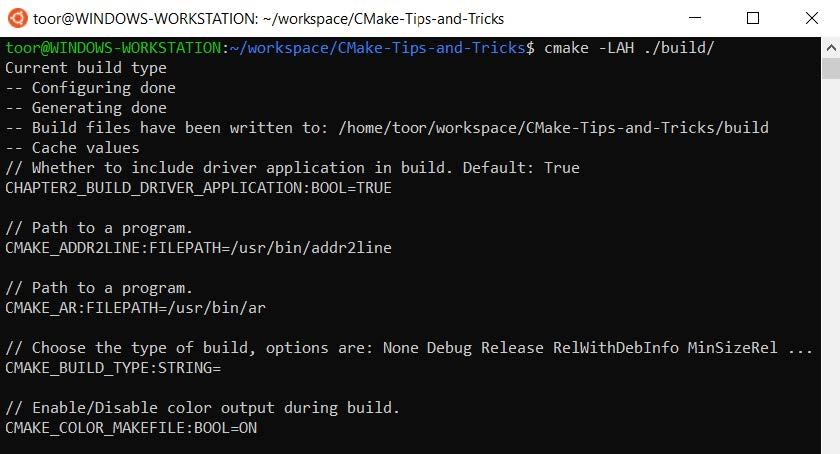
\includegraphics[width=0.8\textwidth]{content/1/chapter2/images/12.jpg}\\
图2.12 CMake转储的缓存变量列表
\end{center}

\hspace*{\fill} \\ %插入空行
\noindent
\textbf{通过CLI构建配置好的项目}

要生成已配置的工程,需要使用\texttt{cmake -{}-build ./build}。这个命令告诉CMake构建已经在构建文件夹中配置的CMake项目。

也可以使用\texttt{cd build \&\& make}进行构建。使用\texttt{cmake -{}-build}的好处是,省去了调用特定于构建系统的命令。在构建CI管道或构建脚本时,可以在不更改构建命令的情况下,更改构建系统生成器。

可以看到\texttt{cmake -{}-build ./build}的输出示例如下所示:

\begin{center}
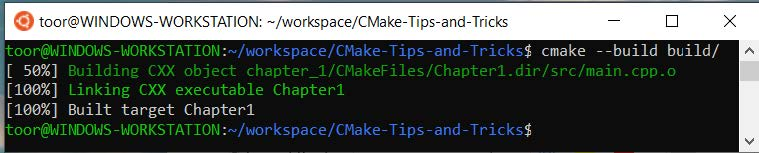
\includegraphics[width=1.\textwidth]{content/1/chapter2/images/13.jpg}\\
图2.13 构建配置好的项目
\end{center}

\hspace*{\fill} \\ %插入空行
\noindent
\textbf{并行构建}

还可以在发出生成命令时,自定义生成时间详细信息。要指定并行构建的任务数,可以在\texttt{cmake -{}-build}中追加\texttt{-{}-parallel <job\_count>}。

要并行构建,请使用\texttt{cmake -{}-build ./build -{}-parallel 2},其中数字2指定了任务数。对于构建系统,建议的任务数最多为每个硬件线程一个作业。多核系统中,还建议至少使用比可用硬件线程数少一个的线程,以避免在构建过程中影响系统的响应能力。

\begin{tcolorbox}[colback=webgreen!5!white,colframe=webgreen!75!black,title=Note]
通常可以在每个硬件线程中使用多个任务,从而获得更快的构建时间,因为构建过程主要受I/O限制,但实际情况可能有所不同,需要进行实验和观察。

此外,某些构建系统(如Ninja)会尝试利用系统中可用的尽可能多的硬件线程,若目标是使用系统中的所有硬件线程,那么为此类构建系统指定任务数就多余了。可以在Linux环境中,使用nproc命令来获取硬件线程计数。
\end{tcolorbox}

在期望在不同环境中调用的命令(如CI/CD脚本和构建脚本)中,不使用环境相关变量的固定值,这是一个很好的实践。下面是一个使用nproc动态确定并行任务数量的构建命令示例:

\begin{tcblisting}{commandshell={}}
cmake --build ./build/ --parallel $(($(nproc)-1))
\end{tcblisting}

让我们观察不同的任务数如何影响构建时间,将使用时间工具来测试每次命令调用的时间。环境如下:

\begin{itemize}
\item 
OS: Ubuntu 20.04.3 LTS (Focal Fossa)

\item 
CPU: AMD Ryzen Threadripper 1950X 16-Core Processor (32线程)

\item 
RAM: 32 GB
\end{itemize}

对于一个任务(\texttt{-{}-parallel 1}),构建时间如下所示:

\begin{center}
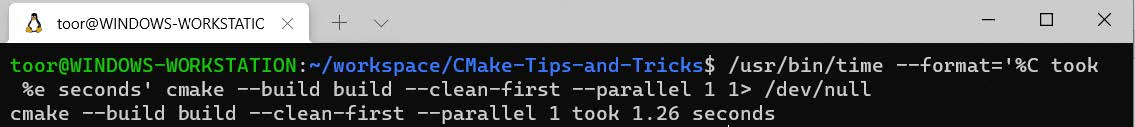
\includegraphics[width=1.\textwidth]{content/1/chapter2/images/14.jpg}\\
图2.14 一个任务的并行构建时间结果
\end{center}

两个任务(\texttt{-{}-parallel 2})的构建时间结果如下:

\begin{center}
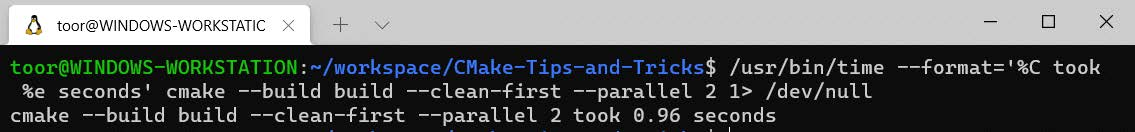
\includegraphics[width=1.\textwidth]{content/1/chapter2/images/15.jpg}\\
图2.15 两个任务的并行构建时间结果
\end{center}

三个任务(\texttt{-{}-parallel 3})的构建时间结果如下:

\begin{center}
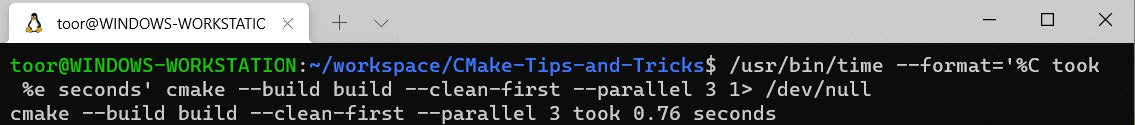
\includegraphics[width=1.\textwidth]{content/1/chapter2/images/16.jpg}\\
图2.16 三个任务的并行构建时间结果
\end{center}

四个任务(\texttt{-{}-parallel 4})的构建时间结果如下:

\begin{center}
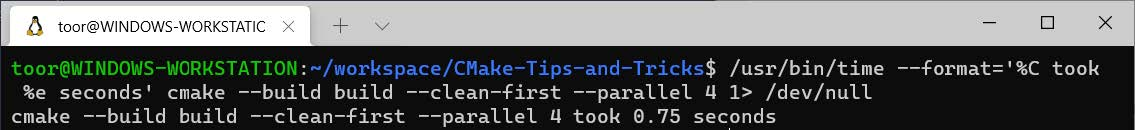
\includegraphics[width=1.\textwidth]{content/1/chapter2/images/17.jpg}\\
图2.17 四个任务的并行构建时间结果
\end{center}

即使是一个非常简单的项目,也可以清楚地看到多个任务并行可以减少构建时间。从一个作业到两个任务减少了0.3秒的构建时间,而从两个任务到三个任务则增加了0.2秒。但是,从3个作业到4个任务只会产生0.01秒的差异,这意味着已经达到了这个项目的构建并行性的极限,增加更多的工作将不会在构建时间上实现显著的差异。

\hspace*{\fill} \\ %插入空行
\noindent
\textbf{只构建特定的目标}

默认情况下,CMake将构建已配置的所有可用目标。由于构建所有目标并不总是理想的,CMake允许通过\texttt{-{}-target}子选项构建目标的子集,子选项可以指定多次:

\begin{tcblisting}{commandshell={}}
cmake --build ./build/ --target "ch2_framework_component1"
--target "ch2_framework_component2"
\end{tcblisting}

该命令将构建范围限制为\texttt{ch2\_framework\_component1}和\texttt{ch2\_framework\_component2}目标。若这些目标也依赖于其他目标,它们也会构建。

\hspace*{\fill} \\ %插入空行
\noindent
\textbf{构建之前删除以前的构建}

若想要运行一个干净的构建,可能想要首先从以前的运行中删除构建。为此,可以使用\texttt{-{}-clean-first}子选项。此子选项将调用一个特殊的目标,该目标清除由构建过程生成的所有构件(例如,调用\texttt{make clean})。

下面是一个示例,说明如何对名为build的构建文件夹执行此操作:

\begin{tcblisting}{commandshell={}}
cmake --build ./build/ --clean-first
\end{tcblisting}

\hspace*{\fill} \\ %插入空行
\noindent
\textbf{调试构建过程}

正如在前面的向编译器传递标志一节中所做的那样,可能希望检查构建过程中使用哪些参数调用了哪些命令。\texttt{-{}-verbose}指示CMake以verbose模式调用所有构建命令,前提是该命令支持verbose模式。这使我们能够轻松地调试讨厌的编译和链接错误。

要在详细模式下构建名为build的文件夹,使用\texttt{-{}-build},示例如下:

\begin{tcblisting}{commandshell={}}
cmake --build ./build/ --verbose
\end{tcblisting}

\hspace*{\fill} \\ %插入空行
\noindent
\textbf{将命令行参数传递给构建工具}

若需要将参数传递给底层构建工具,可以在命令的末尾加上\texttt{-{}-},并输入给定的参数:

\begin{tcblisting}{commandshell={}}
cmake --build ./build/ -- --trace
\end{tcblisting}

\texttt{-{}-trace}将直接传递给构建工具,我们的例子中就是make。这将导致make为构建的每个配方打印跟踪信息。

\hspace*{\fill} \\ %插入空行
\noindent
\textbf{通过CLI安装项目}

CMake允许在环境中进行安装,CMake代码必须使用\texttt{install()}指令来指定当调用\texttt{cmake -{}-install}(或构建系统等效)时安装什么。chapter\_2的内容已经以这样的方式配置用于说明指令。我们将在第4章中学习如何使CMake目标可安装。

\texttt{cmake -{}-install}需要一个已经配置和生成的项目。然后,执行\texttt{cmake -{}-install <project\_binary\_dir>}来安装工程。我们的例子中,build作为一个项目二进制目录,所以<project\_binary\_dir>将被build取代。

示例输出如下图所示:

\begin{center}
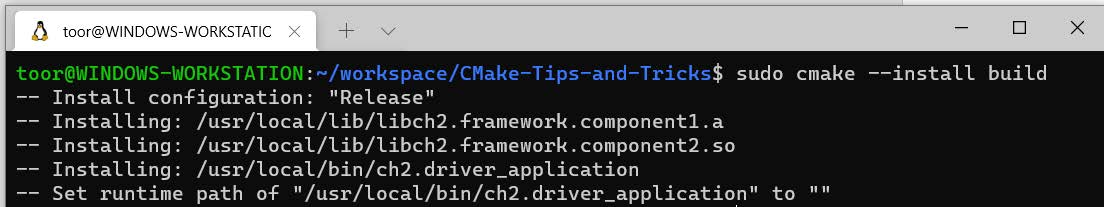
\includegraphics[width=1.\textwidth]{content/1/chapter2/images/18.jpg}\\
图2.18 安装工程
\end{center}

不同环境的默认安装目录不同。对于类Unix环境,默认为\texttt{/usr/local},而在Windows环境中,默认为\texttt{C:/Program Files}。

\begin{tcolorbox}[colback=webgreen!5!white,colframe=webgreen!75!black,title=Tip]
在尝试安装项目之前,必须已经构建了项目。

为了能够成功安装项目,必须拥有适当的权限来写入安装目标目录。
\end{tcolorbox}

\hspace*{\fill} \\ %插入空行
\noindent
\textbf{修改默认安装路径}

要更改默认安装目录,可以指定的\texttt{-{}-prefix}参数,如下所示:

\begin{tcblisting}{commandshell={}}
cmake --install build --prefix /tmp/example
\end{tcblisting}

将安装目录指定为\texttt{/tmp/example},使用\texttt{cmake -{}-install}后,\texttt{/tmp/example}目录下的内容如下图所示:

\begin{center}
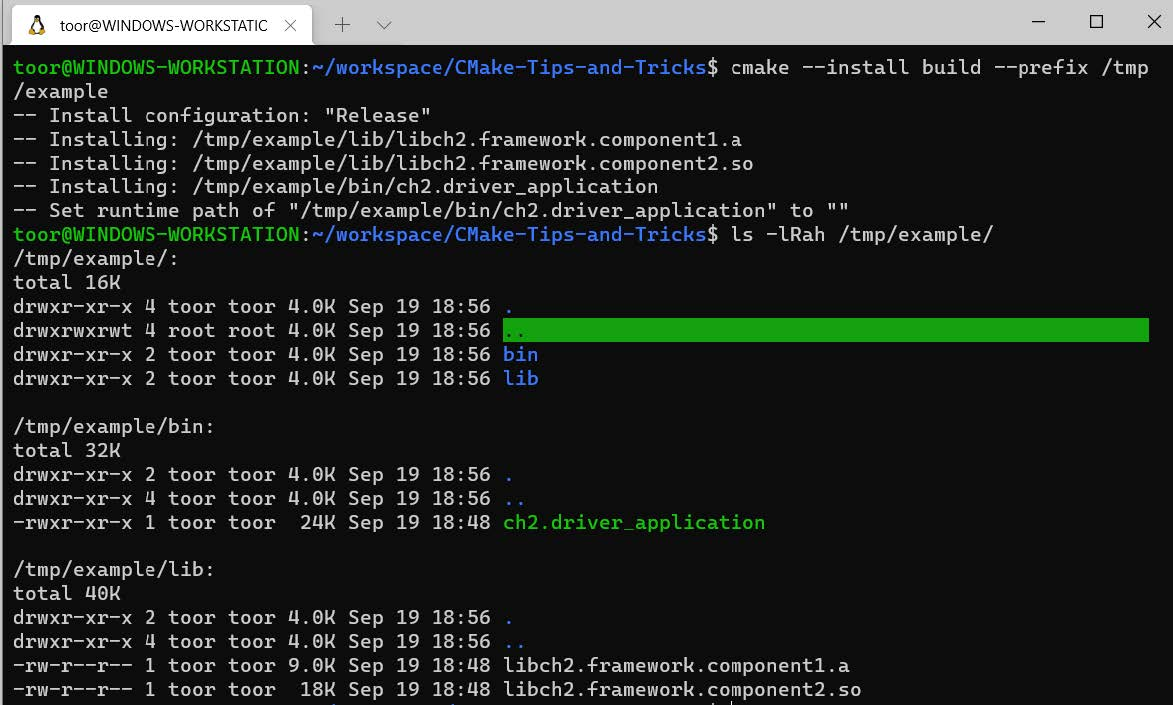
\includegraphics[width=0.8\textwidth]{content/1/chapter2/images/19.jpg}\\
图2.19 将项目安装到不同的路径
\end{center}

可以看到,安装根目录成功更改为\texttt{/tmp/example}。

\hspace*{\fill} \\ %插入空行
\noindent
\textbf{安装时瘦身二进制文件}

软件世界中,构建工件通常与一些额外的信息捆绑在一起,例如:调试所需的符号表。这些信息在执行最终产品时可能不是必需的,并且可能会极大地增加二进制大小。若希望减少最终产品的存储空间,瘦身二进制文件可能是一个不错的选择。瘦身的另一个好处是,这会使逆向工程二进制文件变得更加困难,因为从二进制文件中剥离了基本的符号信息。

CMake的\texttt{-{}-install}允许在安装操作时瘦身二进制文件。可以通过在\texttt{-{}-install}中指定附加的\texttt{-{}-strip}选项来启用,如下所示:

\begin{tcblisting}{commandshell={}}
cmake --install build --strip
\end{tcblisting}

下面的示例中,可以观察未瘦身和瘦身的二进制文件之间的大小差异。注意,瘦身静态库有一些限制,CMake默认情况下不会执行:

\begin{center}
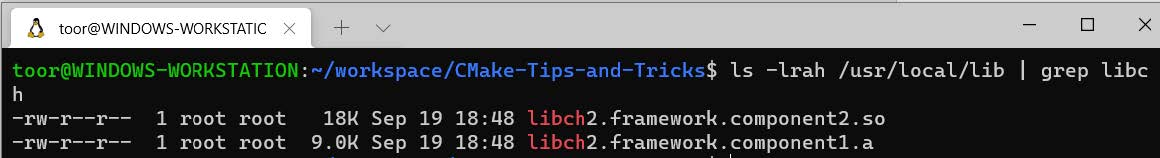
\includegraphics[width=1.\textwidth]{content/1/chapter2/images/20.jpg}\\
图2.20 工件大小(未瘦身)
\end{center}

使用瘦身的(\texttt{cmake - install build -{}-strip})二进制文件,大小差异如下图所示:

\begin{center}
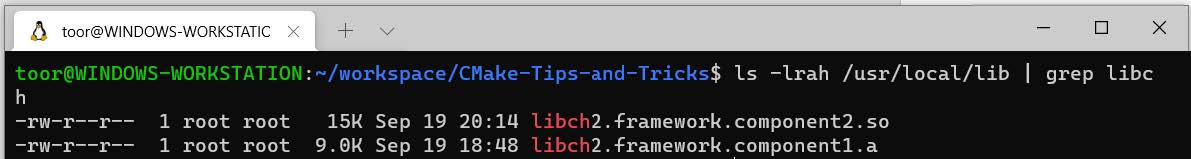
\includegraphics[width=1.\textwidth]{content/1/chapter2/images/21.jpg}\\
图2.21 工件大小(已瘦身)
\end{center}

\hspace*{\fill} \\ %插入空行
\noindent
\textbf{只安装特定组件(基于组件的安装)}

若项目在\texttt{install()}中使用了CMake的\texttt{COMPONENT}特性,可以通过指定组件名称来安装特定的组件。组件特性允许将安装分离为子部分,为了说明这个功能,chapter\_2示例构造成两个组件,分别是库和可执行文件。

为了安装特定的组件,\texttt{cmake -{}-install}需要附加\texttt{-{}-component}参数:

\begin{tcblisting}{commandshell={}}
cmake --install build --component executables
\end{tcblisting}

下面是一个示例:

\begin{center}
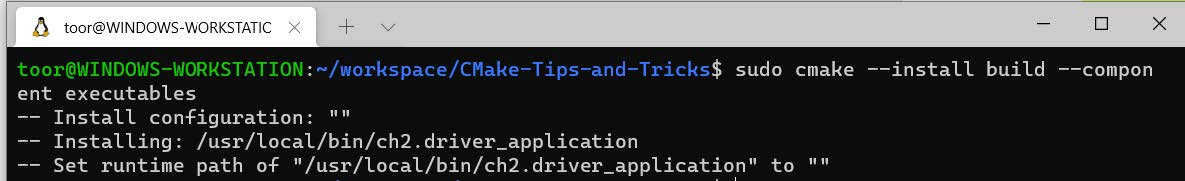
\includegraphics[width=1.\textwidth]{content/1/chapter2/images/22.jpg}\\
图2.22 只安装特定的组件
\end{center}

\hspace*{\fill} \\ %插入空行
\noindent
\textbf{安装特定的配置(仅用于多配置生成器)}

有些生成器支持同一个构建配置的多个配置(例如,Visual Studio)。对于这种类型的生成器,\texttt{-{}-install}选项提供了一个\texttt{-{}-config}参数来指定要安装的二进制文件配置。

这里有一个例子:

\begin{tcblisting}{commandshell={}}
cmake --install build --config Debug
\end{tcblisting}

\begin{tcolorbox}[colback=webgreen!5!white,colframe=webgreen!75!black,title=Note]
示例中使用的命令参数非常长且明确,显式地指定参数允许我们在每次运行中获得一致的结果,无论在哪个环境中运行命令。若没有\texttt{-G}参数,CMake将默认使用环境首选的构建系统生成器。我们的座右铭是:显式总是比隐式好,前者使我们的意图更加清晰,也使CMake代码更容易维护。
\end{tcolorbox}

我们已经介绍了CMake命令行用法的基本原理,继续学习其他可用的交互形式——CMake的图形界面。











